\documentclass{beamer}[10]
\usepackage{pgf}
\usepackage[english]{babel}
\usepackage[utf8]{inputenc}
\usepackage{beamerthemesplit}
\usepackage{graphics,epsfig, subfigure}
\usepackage{url}
\usepackage{srcltx}
\usepackage{hyperref}
\usepackage{enumitem}
\usepackage[round]{natbib}

\definecolor{kugreen}{RGB}{50,93,61}
\definecolor{kugreenlys}{RGB}{132,158,139}
\definecolor{kugreenlyslys}{RGB}{173,190,177}
\definecolor{kugreenlyslyslys}{RGB}{214,223,216}
\setbeamercovered{transparent}
\mode<presentation>
\usetheme[numbers,totalnumber,compress,sidebarshades]{PaloAlto}
\setbeamertemplate{footline}[frame number]
\usecolortheme[named=kugreen]{structure}
\useinnertheme{circles}
\usefonttheme[onlymath]{serif}
\setbeamercovered{transparent}
\setbeamertemplate{blocks}[rounded][shadow=true]
\setbeamercolor{page number in head/foot}{fg=black}
\setbeamerfont{page number in head/foot}{}
\setbeamertemplate{caption}[numbered]


\logo{\includegraphics[width=0.8cm]{figures/umatlogo}}
%\useoutertheme{infolines} 
\title[]{DEVELOPMENT OF AN EFFICIENT PUBLIC TRANSPORT SEARCH PORTAL FOR GHANA}
\author[]{ENOCK SETH NYAMADOR \newline \small{SUPERVISED BY DR HAMIDU ABDEL-FATAO}}
\institute[]{COMPUTER SCIENCE AND ENGINEERING DEPARTMENT \\ UNIVERSITY OF MINES AND TECHNOLOGY}
\date{\today}



\begin{document}
	\frame{\titlepage \vspace{-0.5cm}
	}
	
	\frame
	{
		\frametitle{OVERVIEW}
		\tableofcontents%[pausesection]
	}
	
	\section{Problem Definition}
	
	\frame{
		\frametitle{PROBLEM DEFINITION}
		\large
			\begin{itemize}[label=$ \bullet $]
				\item Road transport is the major means of transportation in Ghana, \citep{aidoo_passengers_2013}.
				\vspace{0.2cm}
				\item Over 95\%  of all passenger and freight traffic and about 97\% of all passenger miles in Ghana is by road, \citep{unesco_transportation:_????}.
				\vspace{0.2cm}
				%\item Vast majority of passengers commuting between places mostly rely on public transport services in the form of privately owned or corporate taxis, \textit{tro tros} (shared minivans), buses commuting between major cities \citep{abane2011travel}
				\item Privately owned or corporate taxis, \textit{tro tros} (shared minivans), buses commuting between major cities, \citep{abane2011travel}.
			\end{itemize}
	}




\frame{
	\frametitle{PROBLEM DEFINITION (CONT'D)}
	\large
	\begin{itemize}[label=$ \bullet $]
		\item The transport industry is currently dominated by the 
		informal sector which provides about 90\% of transport services but their services are unreliable and uncomfortable \citep{bonaventura_assessment_2015}.
		\vspace{0.2cm}
		\item Individually or privately operated transport services are members of unions or associations. These unions and associations serve as regulatory and mouth-piece to each of their members \citep{fouracre1994public}.
		
	\end{itemize}
}


		\frame{
	\frametitle{PROBLEM DEFINITION (CONT'D)}
	\LARGE
	\begin{block}{Challenges}
		\begin{itemize}[label=$ \star $]
\item Difficulty in finding terminals specific location and detailed information.
\vspace{0.3cm}
\item Fares and stations keep changing.
		\end{itemize}
	\end{block}
	
}


	\frame{
		\frametitle{PROBLEM DEFINITION (CONT'D)}
		\begin{block}{Typical Ghanaian Transport Terminal}
					\begin{figure}
					\includegraphics[width=0.7\linewidth]{figures/kaneshe}
					\caption{Kaneshie Transport Terminal}
					\label{fig2:kaneshe}
					\end{figure}
		\end{block}
}
		
	
	\section{Project Objectives}
	\frame{
		\frametitle{PROJECT OBJECTIVES}
		\LARGE
%		\begin{block}{This project seeks to:}
			\begin{itemize}[label=$ \star $]
				\item To develop a web application that provides detailed information about public transport routes in Ghana.
%				\begin{itemize}[label=$ \ast $]
%					\item To mitigate the difficulty in finding transport terminals and improve trip planning
\vspace{0.5cm}
					\item To provide reusable geospatial data on transport terminals.
%				\end{itemize}
			\end{itemize}
%		\end{block}
	}
	

	
	\section{Methodology}
	
	\frame{
		\frametitle{METHODOLOGY}
		\LARGE
%		\begin{block}{Methods used for this project:}
			\begin{itemize}[label=$ \ast $]
				\item Review of related literature
				\vspace{0.5cm}
				\item Conducting feasibility studies
				\vspace{0.5cm}
				\item Requirements gathering and Analysis
				\vspace{0.5cm}
				\item Functional and non-functional requirements
				\vspace{0.5cm}
				\item Performing data Collection
		\end{itemize}
%	\end{block}
	}
		
%	\section{Results and discussion}
%	\frame{
%		\frametitle{RESULTS AND DISCUSSION}
%		\begin{itemize}[label=$ \star $]
%			\item User registers as a student selecting his hall of residence and institution.
%			\item User can purchase any listed product or book any service
%			\item User is able to join the live chat room on the home page of the application
%			\item A user can create his/her own shop and post products,billboards,Events and Personal skill.
%		\end{itemize}
%	}
	
%	\section{Analysis of Existing Systems}
%	
%	\frame{
%		\frametitle{ANALYSIS OF EXISTING SYSTEMS}
%		\begin{block}{	Although there exist systems with similar functionalities as this project, most of these existing systems:}
%		\begin{itemize}[label=$ \ast $]
%			\item Do not suit and focus on the Ghanaian transport system
%			\vspace{0.3cm}
%			\item Lack fare information
%			\vspace{0.3cm}
%			\item Are less reliable; E.g. Word of mouth
%			\vspace{0.3cm}
%			\item Are not frequently updated
%		\end{itemize}
%		\end{block}
%	}

\frame{
	\frametitle{REVIEW OF RELATED LITERATURE}
	\Large
	\begin{itemize}[label=$ \bullet $]
		\item \cite{neumann_toward_2015} have developed the first  minibus supply model based on demand and street network only in South Africa; leading to Taximap: a public transport search web portal
	\end{itemize}
}

	\frame{
	\frametitle{CONDUCTING FEASIBILITY STUDIES}
	\Large
\begin{block}{Areas considered:}
	\begin{itemize}[label=$ \bullet $]
		\item Technical feasibility.
		\vspace{0.5cm}
		\item  Resource feasibility.
		\vspace{0.5cm}
		\item  Operational feasibility.
		\vspace{0.5cm}
		\item  Schedule feasibility.
	\end{itemize}
\end{block}
}
	
	\frame{
	\frametitle{REQUIREMENTS GATHERING AND ANALYSIS}
	\Large
	\begin{block}{Questions that must be answered to ensure that the system can survive:}
		\begin{itemize}[label=$ \star $]		
			\uncover<1->{\item Where is the system going to be used?}
			\uncover<2->{\item Who is going to use the system?}
			\uncover<3->{\item What data should be input into the system?}
			\uncover<4->{\item What Software Development Life Cycle (SDLC) model to be used?}
			\uncover<6->{\item What type of output information will the system give?}
		\end{itemize}
	\end{block}
	
}
	
		\frame{
		\frametitle{DATA COLLECTION}
		\LARGE
		\begin{itemize}[label=$ \ast $]
			\uncover<2->{\item Field survey.}
			\vspace{0.5cm}
			\uncover<3->{\item OpenStreetMap.}
			\vspace{0.5cm}
			\uncover<4->{\item Crowdsourcing.}
		\end{itemize}
		}
		
	\frame{
		\frametitle{FUNCTIONAL AND NON-FUNCTIONAL REQUIREMENTS}
		\begin{block}{}
		\begin{figure}
			\centering
			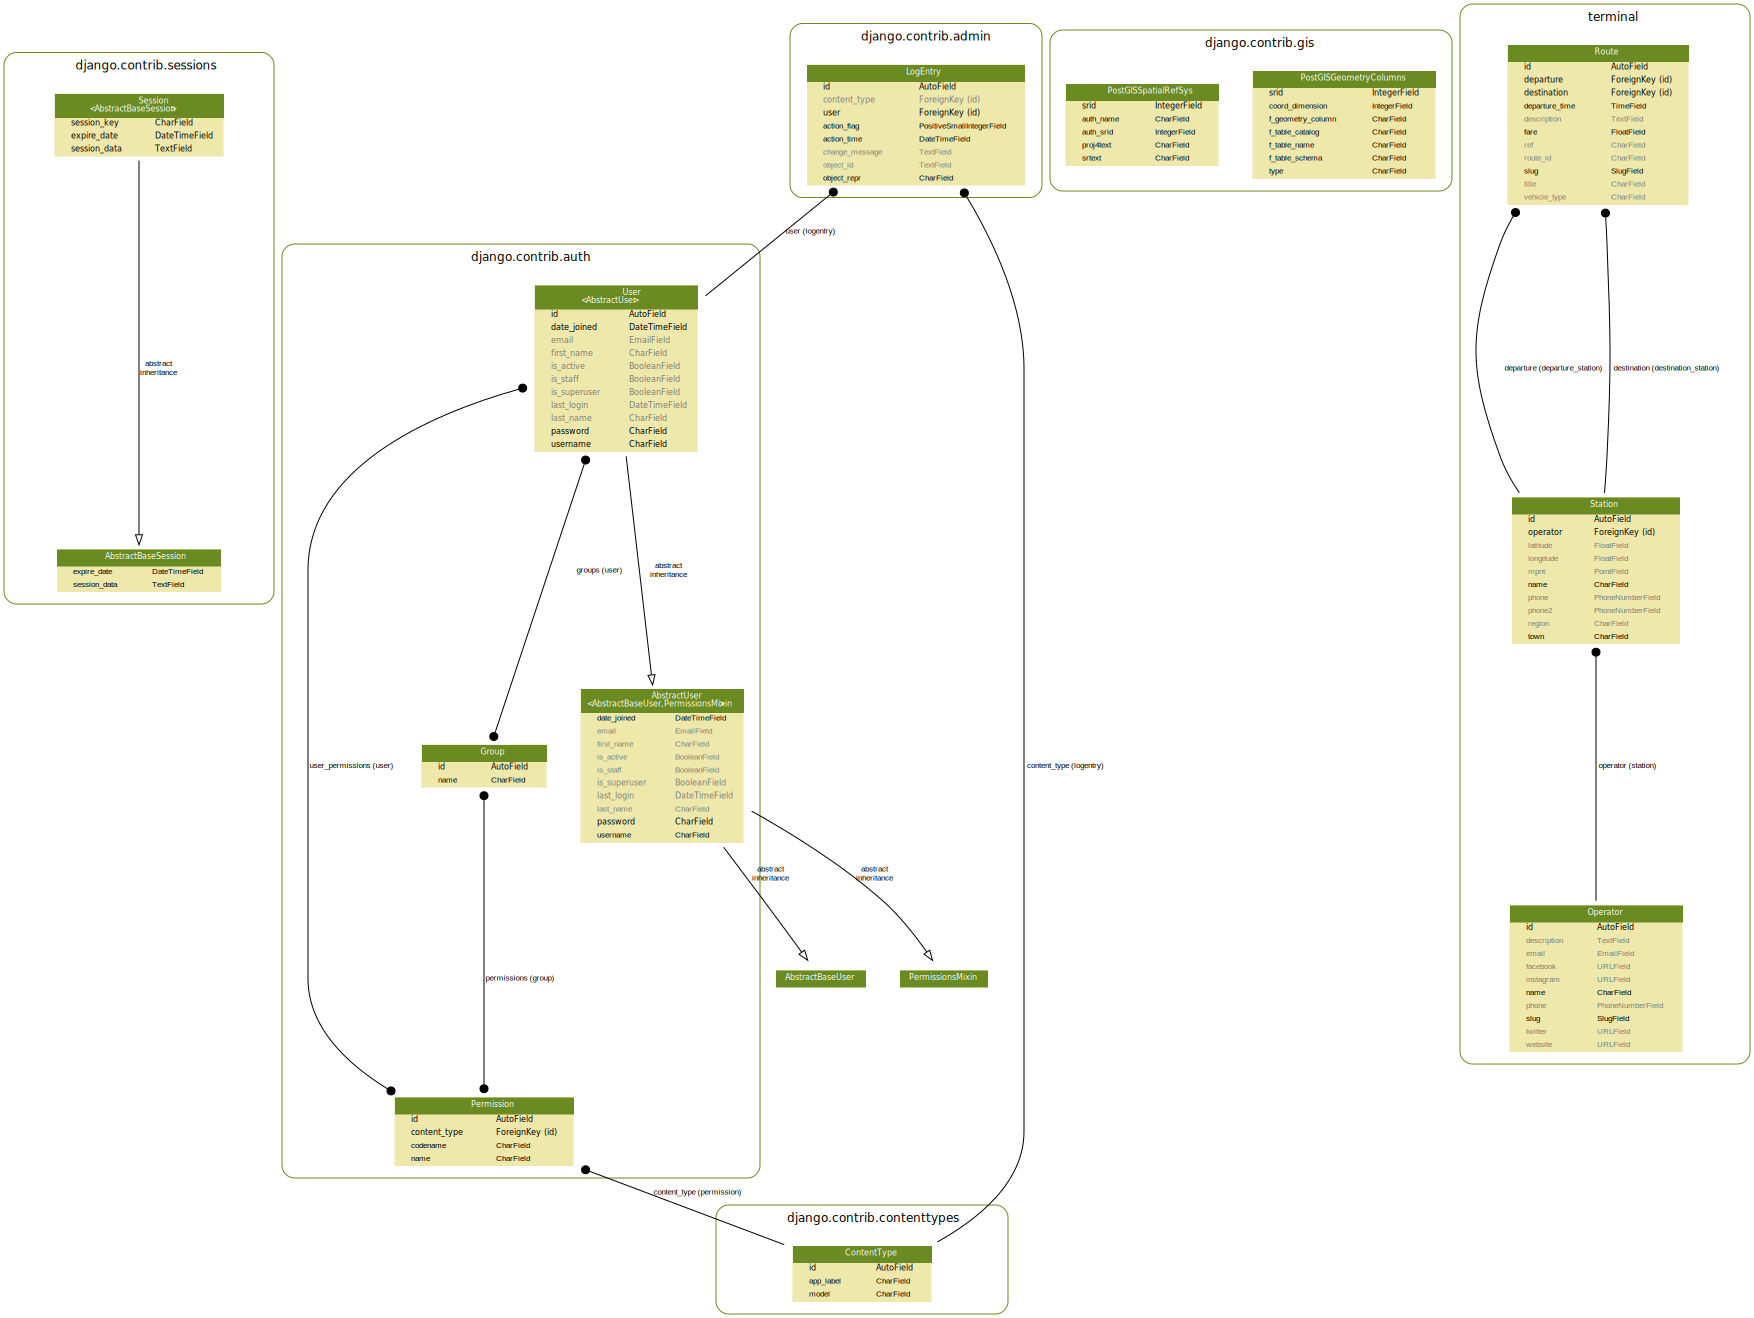
\includegraphics[width=0.8\linewidth]{figures/classdiagram}
			\caption{Class Diagram}
			\label{fig:classdiagram}
		\end{figure}
	\end{block}
		
	}

	\frame{
	\frametitle{FUNCTIONAL AND NON-FUNCTIONAL REQUIREMENTS}
	\begin{block}{}
		\begin{figure}
			\centering
			\includegraphics[width=0.9\linewidth]{figures/usecase}
			\caption{Use Case Diagram}
			\label{fig:usecase}
		\end{figure}
	\end{block}
	
}

	\frame{
	\frametitle{FUNCTIONAL AND NON-FUNCTIONAL REQUIREMENTS}
	\begin{block}{}
		\begin{figure}
			\centering
			\includegraphics[width=0.4\linewidth]{figures/activitydiagram}
			\caption{Activity Diagram}
			\label{fig:activitydiagram}
		\end{figure}
	\end{block}
	
}

%\section{Behavioural Modeling Use Case Diagram}
%\frame{
%	\frametitle{BEHAVIOURAL MODELING USE CASE DIAGRAM}
%
%
%}
%

	\section{Tools Used}

\frame{
	\frametitle{TOOLS USED}
	\large
	%	\begin{block}{The tools used for this project are:}
	\begin{itemize}[label=$ \star $]
		\item Python.
		\vspace{0.2cm}
		\item Django.
		\vspace{0.2cm}
		\item Material Kit.
		\vspace{0.2cm}
		\item PostgreSQL.
		\vspace{0.2cm}
		\item QGIS.
		\vspace{0.2cm}
		\item Leaflet and OpenStreetMap.
		\vspace{0.2cm}
		\item Open Source Routing Machine (OSRM).
		\vspace{0.2cm}
		\item GPS receiver and Smartphone.
	\end{itemize}
	%	\end{block}
}


	\section{Results and Discussions}

\frame{
	\frametitle{RESULTS AND DISCUSSIONS}
	\large
	\begin{block}{The results and discussions:}
		\begin{itemize}[label=$ \star $]
			\item User gets routes based on destination and departure searched.
			\vspace{0.1cm}
			\item A user can access all available operators and view detailed information on each station.
			\vspace{0.1cm}
			\item User can compare fares visually.
			\vspace{0.1cm}
			\item A user is able to access station location in external platform.
			\vspace{0.1cm}
			\item Groups for managing staff privileges.
			\vspace{0.1cm}
			\item Detailed history of changes available in administration dashboard.
			\vspace{0.1cm}
			\item A geospatial database.
		\end{itemize}	
	\end{block}
}

\section{Demonstration}

\frame{
	\frametitle{DEMONSTRATION}
	\centering
	{\Huge GHTP}
}

	\section{Conclusions and Recommendations}

\frame{
	\frametitle{CONCLUSIONS AND RECOMMENDATIONS}
	\large
	\begin{block}{It can be concluded that this system:}
		\begin{itemize}[label=$ \star $]
			\item Will improve trip planning and easy access to information only available within terminals to travellers hence saving time.
			\vspace{0.2cm}
			\item Should be adopted by Ghana Tourism Authority to help tourists find their way around Ghana transport network.
		\end{itemize}	
	\end{block}
\uncover<2->{
	\begin{block}{I would recommend that:}
	\begin{itemize}[label=$ \star $]
		\item Users should be able to book seats from the platform and also support voice input for the visually impaired.
		\vspace{0.2cm}
		\item The system could get users current location and find nearest departure stations for their routes.
	\end{itemize}	
}
\end{block}

}


\frame{

		\small
		\frametitle{REFERENCES}
		\bibliographystyle{agsm}
		\bibliography{references}		

}


\frame{
	\frametitle{}
		\centering
		{\Huge THANK YOU}
}
	
\end{document}
